\chapter{Teilautomatisierte Generierung von Page Objects}
\label{sec:teilautomatisierte_generierung_von_pageObjects}

Ein großer Teil des in Kapitel \ref{sec:probleme_des_page_object_pattern} angesprochenen initialen Mehraufwands bei der Verwendung des Page Object Pattern beläuft sich auf die Erstellung der Page Objects.
Wie in Listing \ref{lst:poCreatePage} und \ref{lst:poShowPage} zu sehen ist, handelt es sich bei Page Objects allerdings um nicht gerade komplexe Klassen. In der Praxis zeigt sich, dass ein Großteil der Arbeit darin besteht die verschiedenen Locatoren der Elemente aus dem Quelltext der Seite herauszufinden und in die Generische Form eines Page Objects zu überführen.
Diese Arbeit kostet zwar viel Zeit, ist allerdings nicht gerade anspruchsvoll.
Möchte man den initialen Mehraufwand bei der Verwendung des Page Object Pattern entgegenwirken bieten die Page Objects somit einen guten Ansatzpunkt.
Ihre Erstellung ist zeitaufwendig und weitestgehend generisch. Gute Voraussetzungen also um das Erzeugen der Pagae Objects zu Automatisieren.
\section{Übersicht über die Idee}
\label{sec:uebersicht_ueber_idee}


Selenium in Verbindung mit dem Page Object Pattern ist auch ein Teil des Technologiestacks des IT-Dienstleisters der Landeshauptstadt München (it@M) und wird dort zum Testen komplexer Webanwendungen verwendet. Auch bei it@M hat man in Bezug auf die Erstellung der Page Objects die Erfahrungen gemacht, dass es sich um eine generische und zeitaufwendige Arbeit handelt.
In Zusammenarbeit mit it@M wurde daher die Idee entwickelt, das Erstellen von Page Objects mit Hilfe einer Softwarelösung zu unterstützen. 
Anhand des Seitenquelltextes der zu testenden Webanwendung sollen die verschiedenen Elemente des Page Objects identifiziert und zur Generierung der Page Objects verwendet werden.
Zwei Ansätze wurden dabei diskutiert. Eine vollautomatisierte Generierung von Page Objects und eine teilautomatisierte Generierung.
Ein vollautomatischer Ansatz würde beinhalten, dass für einen übergebenen Seitenquelltext ohne weiteres Zutun ein vollständiges Page Object generiert wird. Dieser Ansatz hat jedoch mit zahlreichen Problemen zu kämpfen. Oft wird nur ein Bruchteil der Elemente einer Webseite für die Testfälle benötigt. Selenium kann aber prinzipiell jedes Element, dass im Seitenquelltext bereitgestellt wird, ansprechen. Bei einer vollautomatischen Generierung müssten daher entweder alle Elemente einer Seite übernommen oder eine definierte Auswahl getroffen werden.
Wird eine Auswahl getroffen besteht das Risiko, dass Elemente ausgelassen werden die vom Tester möglicherweise benötigt werden. Werden alle Elemente übernommen, werden die Page Objects schnell überladen und unübersichtlich. Das Überladen der Page Objects geschieht dann auf Kosten der Robustheit. Strukturelle Änderungen in der Website wirken sich auch auf die Locatoren der Elemente in den Page Objects aus. Um die Page Objects stabil zu halten, müssen diese bei Änderungen in der Seitenstruktur berichtigt werden.
Es ist daher nicht sinnvoll Elemente in den Page Objects zu pflegen, die nicht verwendet werden. Unbenutzte Elemente bedeuten entweder zusätzlichen Wartungsaufwand oder veralten unbemerkt.
Ein weiteres Problem des vollautomatischen Ansatzes stellen die Übergänge zwischen den Seiten einer Webanwendung dar. Interaktionen mit der Webanwendung wie beispielsweise das betätigen eines Button führen oft zum aufrufen einer neuen Seite. Im weiteren werden diese Übergänge als Transitions bezeichnet. Diese Transitions werden optimaler weise auch in den Page Objects abgebildet. Das Page Object gibt dazu das entsprechende Page Object der Zielseite als Rückgabe eines Methodenaufrufs zurück, wie es beispielsweise in der Methode createEntry() im Listing \ref{lst:poCreatePage} gezeigt ist. Allein aus dem Seitenquelltext zu ermitteln welche Seite das Ziel einer Transition ist erweist sich jedoch oft als sehr schwierig bis unmöglich.
Um die Komplexität des Projektes auf Grund der genannten Probleme nicht zu groß werden zu lassen wurde sich für einen teilautomatisierte Lösung entschieden.
Ziel ist es also nicht, automatisch ein vollständiges Page Object zu generieren sondern den Entwickler bei der Generierung der Page Objects zu unterstützen. Anhand des Quelltextes sollen dem Entwickler die möglichen Elemente der Seite in einer Vorauswahl bereitgestellt werden. Aus diesen Elementen können dann diejenigen ausgewählt werden, die vom Entwickler im späteren Page Object benötigt werden. Auf diese Weise wird eine Überladung der Page Objects verhindert und gleichzeitig sichergestellt, dass die Elemente vorhanden sind, die benötigt werden.
Ob es sich bei einem Element um eine Transition handelt, also ein Element welches auf eine neue Seite führt, muss auch nicht mehr automatisch anhand des Quelltextes ermittelt werden sonder kann vom Entwickler direkt bei der Auswahl der benötigten Elemente mit angegeben werden.
Die so vom Entwickler ausgewählten Informationen können dann verwendet werden um daraus das fertige Page Object zu generieren.
Im Rahmen des Projektes SeleniPo soll dieser Ansatz in Zusammenarbeit mit it@M in Form einer Denktopanwendung umgesetzt werden. 

\section{Abgrenzung zu bestehenden Ansätzen}
\label{sec:abgrenzung_zu_bestehenden_ansaetzen}
Sowohl für die vollautomatische Generierung von Page Objects als auch für eine teilautomatisierten Generierung gibt es bereits mögliche Lösungsansätze. 
Stocco et al. \cite{stocco_why_2015} beschreiben in einem Paper das von ihnen entwickeltes Framework APOGEN mit deren Hilfe Page Objects vollautomatisch generiert werden können. Die Generierung der Page Objects soll dabei weit über das Anlegen von Elementen hinausgehen und auch die Funktionalitäten der einzelnen Webseiten in Form von Methoden mit einschließen.
Das Framework analysiert dazu die Struktur der Webanwendung mittels eines Crawlers. Die Informationen die über den Crawler zusammengetragen wurden, wie beispielsweise das DOM der einzelnen Webseiten, werden anschließend über eine statische Analyse aufbereitet und für die Generierung der Page Objects verwendet.
Nach eigenen Angaben sollen ca. 75\% des von APOGEN generierten Codes ohne Anpassungen verwendet werden können. Die restlichen 25\% benötigen nur kleine Änderungen.
Bei APOGEN handelt es sich jedoch um ein noch sehr junges Projekt. Das Paper zu diesem Projekt wurde im Mai 2015 veröffentlicht. APOGEN ist daher eher einen Prototyp der zwar die Möglichkeiten aufzeigt die in diesem Bereich gegeben sind jedoch noch nicht für den produktiven Einsatz in einem großen unternehmen geeignet ist.
Nach eigenen Angaben Leidet das Projekt noch unter einigen Einschränkungen. Eine der genannten Einschränkungen ist die Limitierung durch den Crawler.
APOGEN kann nur Webseiten in Page Objects umwandeln, die auch durch den Crawler erreicht wurden.
Für einfache Webanwendungen stellt das kein großes Problem da, für sehr komplexe Anwendungen mit einer ausgeprägten logischen Validierung allerdings schon.
Viele Seiten die hinter logisch validierten Eingaben liegen können vom Crawler nicht erreicht werden und stehen somit für die Generierung nicht zur Verfügung.

Neben der vollautomatischen Generierung existieren noch eine Reihe von Open-Source-Framworks 
die einen teilautomatisierten Ansatz verfolgen, ähnlich wie es das Projekt SelneiPo erreichen will.
Stocco et al. \cite{stocco_why_2015} nennen in ihrem Paper die drei derzeit wichtigsten Vertreter:

\begin{itemize}
\item \textit{OHMAP} \cite{virtuetech_gmbh_ohmap_2015}: Bei OHMAP handelt es sich um eine online Webseite die es dem Benutzer erlaubt HTML-Code in eine Textarea zu Kopieren. Aus dem übergebenen HTML-Code generiert das Tool eine einfache Java-Klasse die für jedes gefundene Input-Feld ein WebElement enthält. Die Variablennamen werden dabei aus den HTML-Attributen gebildet. Als Locator wird ein einfacher XPath-Ausdruck verwendet.
	
\item \textit{SWD Page Recorder} \cite{dmytro_zharii_dzharii/swd-recorder_2015}: Der SWD Page Recorder ermöglicht es dem Benutzer eine beliebige Webanwendung zu starten und das GUI der Anwendung mit einem click\&record-Mechanismus zu inspizieren.
Nach jedem Klick auf das Interface der Anwendung wird ein drop-down-Menü angezeigt in welches manuell ein Name für das ausgewählte Element angegeben werden kann. Als Locator wird ein einfacher XPath-Ausdruck generiert.
Das so erstellte Modell der Anwendung kann in verschiedene Sprachen exportiert werden, wie beispielsweise Java, C\#, Rython, Ruby oder Perl. Beim SWD Page Recorder handelt es sich um eine .NET Anwendung.

\item\textit{ WTF PageObject Utility Chrome Extension} \cite{daniel_wiredrive/wtframework_2015}: WTF unterstützt den Entwickler beim erstellen von Page Objects indem Locatoren der Form id, name, CSS oder XPath erstellt werden. Der generierte Code ist in Python.
	
\end{itemize}

Der Technologiestack von it@M sieht eine Entwicklung der Selenium-Testfälle in Java vor. Als Betriebssystem kommt darüber hinaus Linux zum Einsatz.
Zwei der genannten Lösungsansetzen scheiden daher von vornherein für den produktiven Einsatz beim externen IT-Dienstleister der Landeshauptstadt München aus. Beim SWD Page Recorder handelt es sich um eine .NET Anwendung die nur schwer unter Linux betrieben werden kann. Die WTF PageObject Utility Chrome Extension kann nur im Python-Umfeld betrieben werden. OHMAP wäre aus technischer Sicht eine mögliche Lösungsalternative. Allerdings sind Komfort und Umfang der Anwendung aus sicht von it@M nicht ausreichend. Ohne eigne Konfiguration ist es mit OHMAP nur möglich input-Felder zu extrahieren.
Der HTML-Quelltext muss händisch aus der zu testenden Anwendung extrahiert werden. \\
OWAP als auch der SWD Page Recorder haben zusätzlich das Problem, dass die erzeugten XPath ausdrücke oft sehr einfach gewählt werden und damit sehr stark von der Position der Element innerhalb der Seite abhängig sind. Die eigentlichen Charakteristika der Elemente werden somit oft nicht beachtet. Listing \ref{lst:badXPath}
zeigt einen solche von OHMAP generierten XPath.

\begin{lstlisting}[caption={Exportierte Testfälle},label={lst:badXPath}]
	public class YourPageObjectName {
		//...		
 		@FindBy(xpath = "/html/body/div/div[1]/div[1]/h1/a[2]")
		public WebElement followVirtuetechGmbH;	
		//...
	}
\end{lstlisting}

Der zu adressierende Link in  Listing \ref{lst:badXPath} wird alleine über seine Position innerhalb des DOM der Seite bestimmt.
Um den Locator zu zerstören würde es alleine genügen ein weiteres div-Tag vor dem Link einzufügen.
\\
Ein weiteres Problem, dass sich die gezeigten Lösungen teilen ist, dass sie immer nur ein Page Object auf einmal betrachten. Transitionen, also Übergänge zwischen den einzelnen Webseiten der zu testenden Anwendung, werden somit nicht beachtet. Die dynamische Komponente der Anwendung wird beim generieren der Page Objects somit außer acht gelassen und muss nachträglich händisch hinzugefügt werden.

Mit SeleniPo soll der Versuch unternommen werden die Schwachstellen der bereits existierenden Lösungsansätzen zu verbessern und eine Plattformunabhängige Lösung zu schaffen, die in der IT-Infrastruktur von it@M betrieben werden kann.

\newpage
\section{SeleniPo - PageObject Generator}
\label{sec:selenipo_pogenerator}

Abbildung \ref{fig:poGenerator} zeigt die Denktopanwendung (PageObject Generator) die im Rahmen des Projektes SeleniPo entwickelt wurde. Mit Hilfe dieser Anwendung ist es möglich Page Objects teilautomatisiert zu generieren. Die Anwendung bietet dazu die Möglichkeit einen Browser zu starten und über vorgefertigte Selektoren die Webanwendung nach benötigten Elementen bzw. Transitionen zu durchsuchen. Auf diese Weise kann ein Modell der Anwendung erstellt werden, dass zur Generierung der Page Objects verwendet wird.

\begin{figure}[htb]
  \centering  
  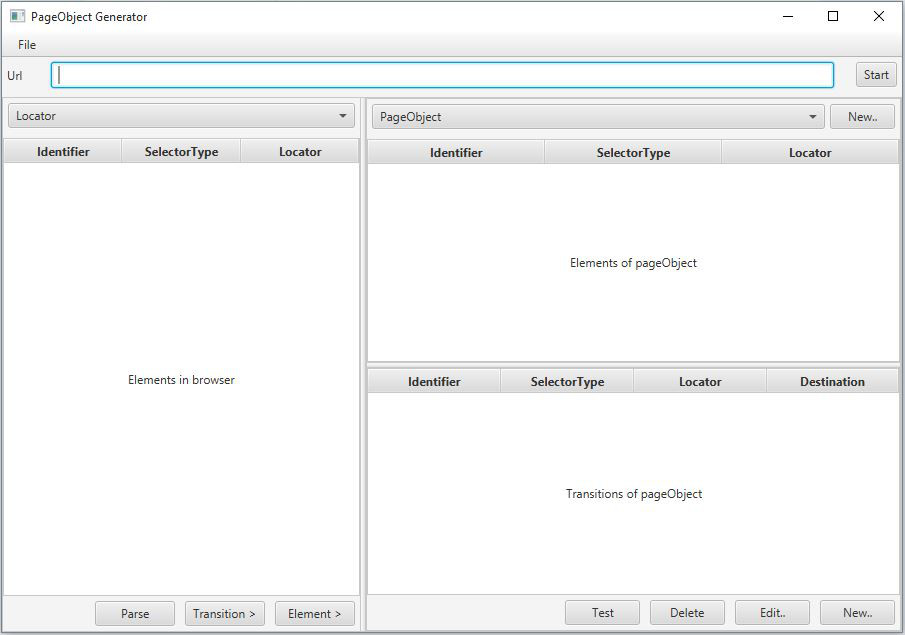
\includegraphics[scale=0.5]{img/poGenerator.JPG}\\
  \caption{SeleniPo - PageObject Generator}
  \label{fig:poGenerator}
\end{figure}



Das Interface des PageObject Generators teilt sich in drei Bereiche:

\begin{itemize}
	\item Das aktuelle Page Object Modell (Abbildung \ref{fig:poGeneratorPo})
	\item Den HTML-Parser (Abbildung \ref{fig:poGeneratorHtml})
	\item Das Menü (Abbildung \ref{fig:poGeneratorMenu})
\end{itemize}


Abbildung \ref{fig:poGeneratorPo} zeigt den Bereich des Generators mit dem das aktuelle Page Object Modell der zu testenden Anwendung verwaltet werden kann. Mit diesem Bereich der Anwendung können neue Page Objects angelegt und bearbeitet werden. Elemente und Transitionen können manuell hinzugefügt, editiert oder gelöscht werden. Darüber hinaus bietet Die Anwendung die Möglichkeit existierende Elemente und Transitionen auf ihre Richtigkeit zu testen.

\begin{figure}[htb]
  \centering  
  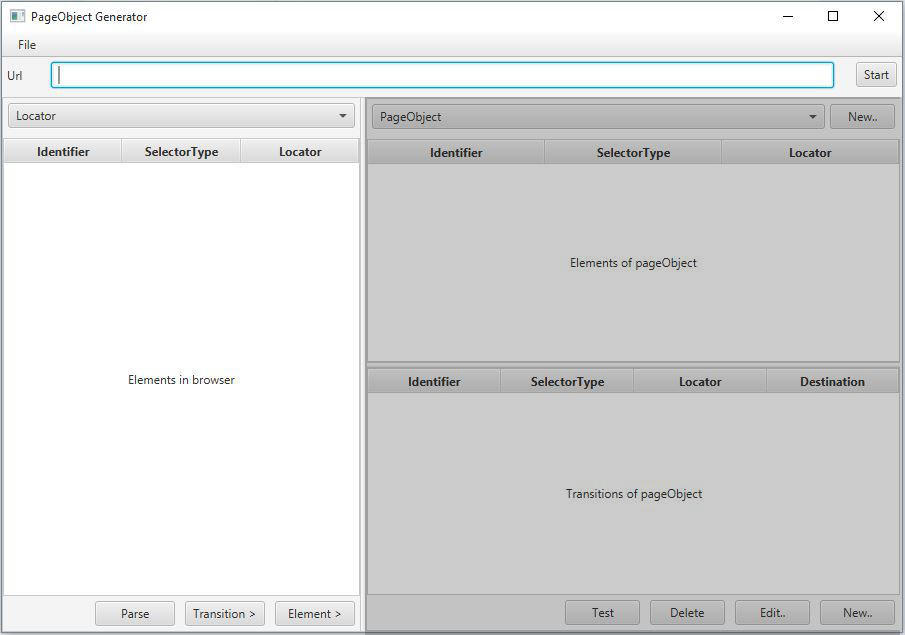
\includegraphics[scale=0.5]{img/poGeneratorPo.JPG}\\
  \caption{SeleniPo - PageObject Generator - Page Object Model}
  \label{fig:poGeneratorPo}
\end{figure}

\newpage

Abbildung \ref{fig:poGeneratorHtml} zeigt den Bereich des Generators mit dem der Entwickler bei der Erstellung von Elementen und Transitionen im Page Object unterstützt werden kann.
Über den Button Start kann ein Browser gestartet werden. Über das Locator-Dropdown kann dann über vorgefertigte Selektoren die aktuell im Browser dargestellte Webseite nach Elementen bzw. Transitionen durchsucht werden. Im Page Object benötigte Elemente und Transitionen können dann in das ausgewählte Page Object im Page Object Modell übernommen werden.

\begin{figure}[htb]
  \centering  
  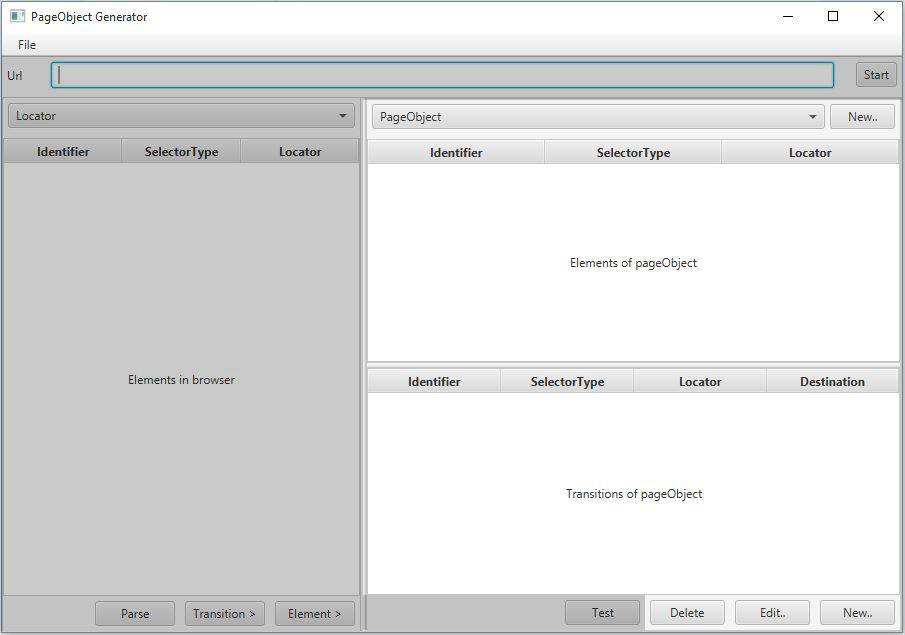
\includegraphics[scale=0.5]{img/poGeneratorHtml.JPG}\\
  \caption{SeleniPo - PageObject Generator - Html Parser}
  \label{fig:poGeneratorHtml}
\end{figure}

\newpage

Abbildung \ref{fig:poGeneratorMenu} markiert das Menü des PageObject Generator. Mit Hilfe des Menüs können Zwischenstände des Page Object Modells gespeichert und geladen werden.
Über das Menü kann darüber hinaus die Generierung der Page Objects aus dem aktuell geladenen Modell gestartet werden.

\begin{figure}[htb]
  \centering  
  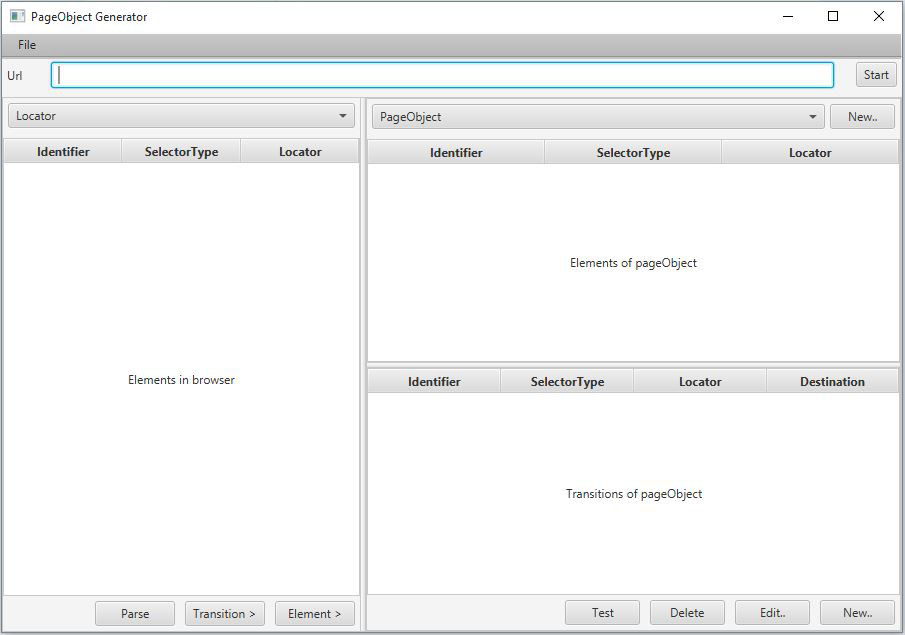
\includegraphics[scale=0.5]{img/poGeneratorMenu.JPG}\\
  \caption{SeleniPo - PageObject Generator - Menü}
  \label{fig:poGeneratorMenu}
\end{figure}

\subsection{Deploymentsicht}

\label{sec:deploymentsicht}
\begin{figure}[htb]
  \centering  
  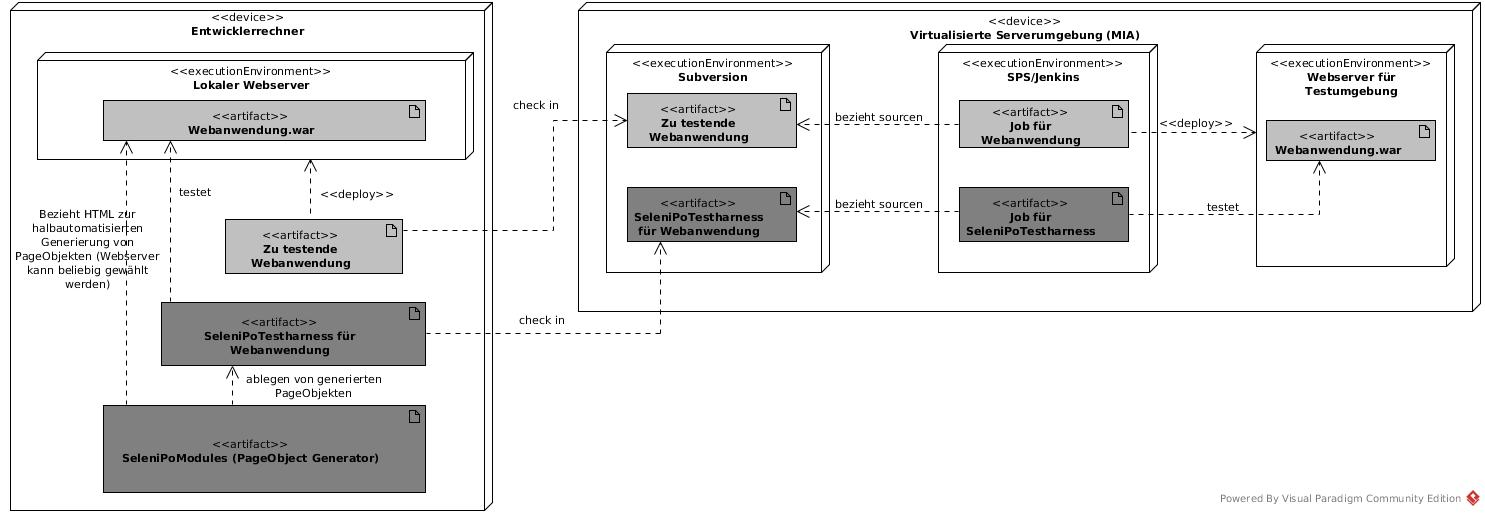
\includegraphics[scale=0.32]{img/Deployment.jpg}\\
  \caption{Einordnung des PageObject Generator in die Deploymentsicht}
  \label{fig:deployment}
\end{figure}

Abbildung \ref{fig:deployment} zeigt die Einordnung des PageObject Generator in die Infrastruktur von it@M. Anhand dieser Abbildung soll gezeigt werden in welchem Bezug sich der Generator zu einer zu testenden Webanwendung befindet.
Zwei übergeordnete Teilbereiche werden unterschieden. Die virtualisierte Serverumgebung (MIA) und der lokale Rechner eines Entwicklers. Auf der virtualisierten Serververumgebung werden die entwicklerübergreifenden Infrastrukturkomponenten wie beispielsweise eine Versionsverwaltung bereitgestellt. Unter dem Entwicklungsrechner ist der Arbeitsplatz eines einzelnen Projektteilnehmers zu verstehen.\\
Auf dem Entwicklungsrechner wird die zu testende Webanwendung entwickelt. Zu Testzwecken kann diese Anwendung in ihrem aktuellen Entwicklungsstand auf einem lokalen Webserver deployt werden.
Der lokale Rechner des Entwicklers ist auch der Ort an dem der PageObject Generator eingesetzt wird. Die lokal deployte Webanwendung kann verwendet werden um für die verschiedenen Seiten der zu testenden Anwendung Page Objects mit Hilfe des Generators zu erzeugen. Diese Page Objects werden bei der Generierung in ein zweites Projekt abgelegt, in welchem die Seleniumtestfälle entwickelt werden. Dieses Projekt wird in Abbildung \ref{fig:deployment} als SeleniPoTestharness bezeichnet und kann vom Entwicklerteam entweder selbst erstellt oder als leeres Quickstart-Projekt vorgefertigt bezogen werden. MIt Hilfe der Page Objects im Testharness können Testfälle entwickelt werden die während der Erstellung auf dem lokalen Entwicklungsrechner gegen die lokal deployte Webanwendung ausgeführt werden.
Der Sourcecode der zu testende Webanwendung als auch des SeleniPoTestharness wir in einer Versionsverwaltung in der virtualisierten Severumgebung abgelegt. Bei it@M wird zu diesem Zweck Subversion eingesetzt. Über die Versionsverwaltung kann eine Softwareproduktionsstraße bedient werden die das bauen, deployen und testen der der Webanwendung automatisiert. Bei it@M kommt hierfür der Continuous Integration Server Jenkins zum Einsatz. Jenkins bezieht die jeweils aktuellen Sourcen für das Testprojekt und die Webanwendung aus dem Subversion und kann so regelmäßig eine Aktuelle version des Webanwendung bauen und auf ein Testsystem in der virtuellen Serverumgebung deployen. Der aktuelle Testharness kann dann analog von Jenkins gesteuert die aktuell entwickelten Selenium Testfälle gegen diesen Webserver zur Ausführung bringen.



\subsection{Fachliche Sicht}
\label{sec:fachliche_sicht}

Abbildung \ref{fig:sequenz} zeigt auf hoher Abstraktionsebene einen Standartablauf bei der Benutzung des Page Object Generators.

\begin{figure}[htb]
  \centering  
  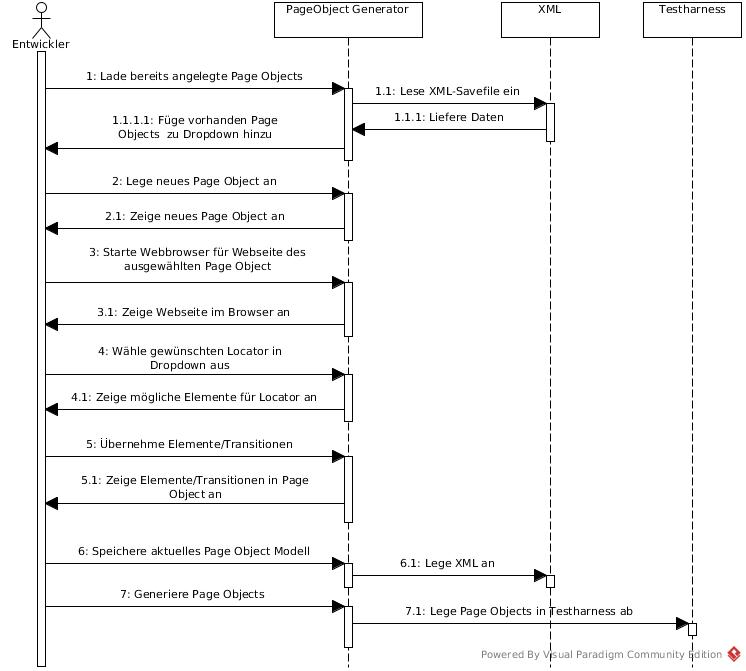
\includegraphics[scale=0.5]{img/Sequenzdiagramm.jpg}\\
  \caption{Ablauf eines Standartanwendungsfall}
  \label{fig:sequenz}
\end{figure}

\newpage


Use-Cases: Beschreibe Standartusecase mit Sequenzdiagramm. (Pageobjekte anlegen -> kann um Elemente und Transitiionen Erweitert werden. Diese können auch Teilautomatisiert aus HTML generiert werden.

Use-Cases Diagramm 
Verbindung von Use-Case-Diagramm mit GUI

--> die einzelnen Usecases fachlich beschreiben.

Technische Sicht. 
Komponentendiagramm Allgemein erklären.

Jede Komponente abarbeiten in sinnvoller tiefe (z.B. Klassendiagram / Zustandsautomat ect.)









\section{übersicht über Aufbau des Systems}

\subsection{pro modul ein kapitel}

\section{Vorteile und Probleme}

\section{Anwendung}
